\begin{figure}[h]
    \centering
    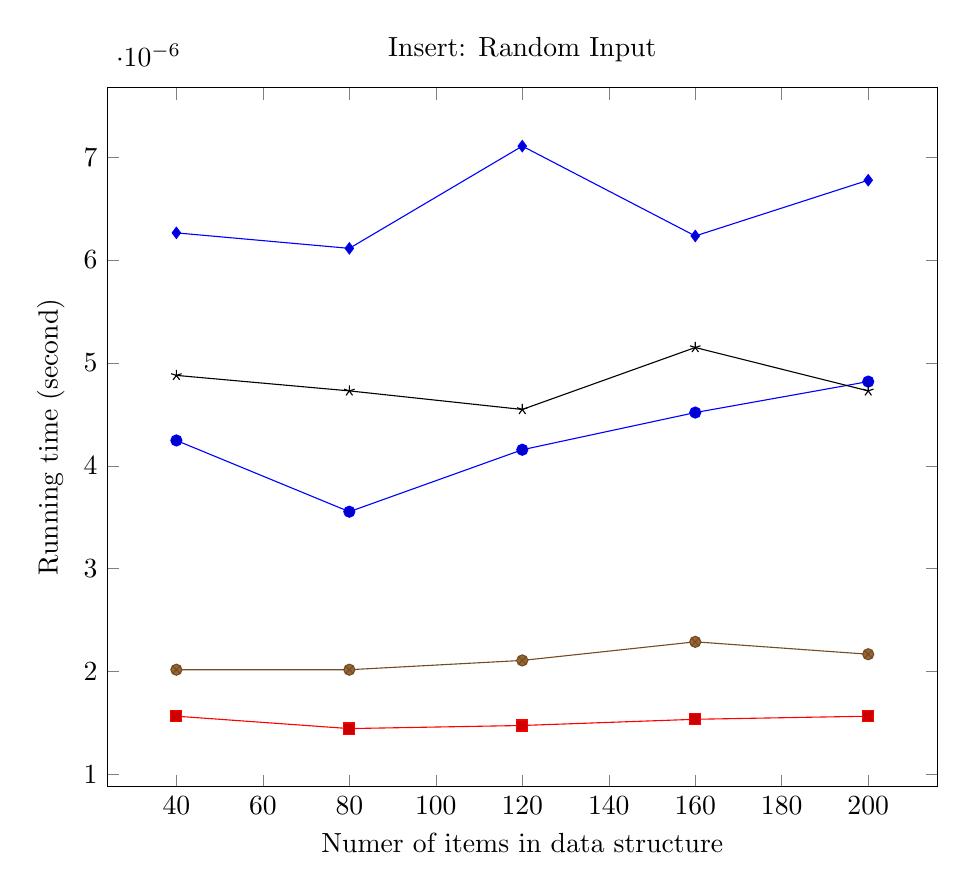
\begin{tikzpicture}
        \begin{axis}[
            xlabel={Numer of items in data structure},
            ylabel={Running time (second)},
            title={Insert: Random Input},
            width=\textwidth
        ]
		\addplot coordinates {
			(40, 4.246572248334246e-06)
			(80, 3.5538689736824836e-06)
			(120, 4.156219646844761e-06)
			(160, 4.517630051381616e-06)
			(200, 4.818805388140391e-06)
		};
		\addplot coordinates {
			(40, 1.566111751216681e-06)
			(80, 1.4456416163710629e-06)
			(120, 1.4757591500824673e-06)
			(160, 1.5359942171500052e-06)
			(200, 1.566111751216681e-06)
		};
		\addplot coordinates {
			(40, 2.0178747565324785e-06)
			(80, 2.017874756177207e-06)
			(120, 2.1082273573114206e-06)
			(160, 2.2889325592245767e-06)
			(200, 2.1684624243789584e-06)
		};
		\addplot coordinates {
			(40, 4.879040455207928e-06)
			(80, 4.728452787006176e-06)
			(120, 4.54774758509302e-06)
			(160, 5.150098258255298e-06)
			(200, 4.728452787006176e-06)
		};
		\addplot coordinates {
			(40, 6.264447004511453e-06)
			(80, 6.11385933595443e-06)
			(120, 7.107737947364967e-06)
			(160, 6.234329470800048e-06)
			(200, 6.776445076894788e-06)
		};
        \legend{}
        \end{axis}
    \end{tikzpicture}
    \caption{Average of 0 operations, benchmarked every 0, starting at 0.}
\end{figure}